\documentclass[10pt,a4paper]{report}
\usepackage[utf8]{inputenc}
\usepackage{amsmath}
\usepackage{amsfonts}
\usepackage{amssymb}
\usepackage{graphicx}
\usepackage{lmodern}
\usepackage{listings}
\usepackage[left=2cm,right=2cm,top=2cm,bottom=2cm]{geometry}
\usepackage{color}
\usepackage{float}
\definecolor{mygreen}{rgb}{0,0.6,0}
\definecolor{mygray}{rgb}{0.5,0.5,0.5}
\definecolor{mymauve}{rgb}{0.58,0,0.82}

\lstset{ %
  backgroundcolor=\color{white},   % choose the background color; you must add \usepackage{color} or \usepackage{xcolor}
  basicstyle=\footnotesize,        % the size of the fonts that are used for the code
  breakatwhitespace=false,         % sets if automatic breaks should only happen at whitespace
  breaklines=true,                 % sets automatic line breaking
  captionpos=b,                    % sets the caption-position to bottom
  commentstyle=\color{mygreen},    % comment style
  deletekeywords={...},            % if you want to delete keywords from the given language
  escapeinside={\%*}{*)},          % if you want to add LaTeX within your code
  extendedchars=true,              % lets you use non-ASCII characters; for 8-bits encodings only, does not work with UTF-8
  frame=single,                    % adds a frame around the code
  keepspaces=true,                 % keeps spaces in text, useful for keeping indentation of code (possibly needs columns=flexible)
  keywordstyle=\color{blue},       % keyword style
  language=Octave,                 % the language of the code
  morekeywords={*,...},            % if you want to add more keywords to the set
  numbers=left,                    % where to put the line-numbers; possible values are (none, left, right)
  numbersep=5pt,                   % how far the line-numbers are from the code
  numberstyle=\tiny\color{mygray}, % the style that is used for the line-numbers
  rulecolor=\color{black},         % if not set, the frame-color may be changed on line-breaks within not-black text (e.g. comments (green here))
  showspaces=false,                % show spaces everywhere adding particular underscores; it overrides 'showstringspaces'
  showstringspaces=false,          % underline spaces within strings only
  showtabs=false,                  % show tabs within strings adding particular underscores
  stepnumber=2,                    % the step between two line-numbers. If it's 1, each line will be numbered
  stringstyle=\color{mymauve},     % string literal style
  tabsize=2,                       % sets default tabsize to 2 spaces
  title=\lstname                   % show the filename of files included with \lstinputlisting; also try caption instead of title
}
\author{Yapi Donatien Achou}
\title{Non linear diffusion equation}
\begin{document}

\maketitle
\section{Introduction}
In this project we solve the time dependent non linear diffusion equation, with Neumann boundary condition.
To formulate a finite element method for the non linear diffusion equation, the time derivative is approximated by the backward scheme. The nonlinear diffusion equation is thus sampled at some time level say $k$ and expressed as a spatial problem. The nonlinear term in the diffusion equation is linearised by using a Picard iteration.\\
The discretised equation is implemented in FEniCs. Fenics is a user friendly software for solving finite element method. The first verification of the FEniCs implementation reproduce a constant solution. The second verification of the FEniCs implementation reproduce a simple analytical solution and shows that the ratio of the error and the time step is constant. The nonlinear FEniCs implementation is tested by recovering the convergence rate of the backward Euler scheme. The project is conclude by simulating a nonlinear Gaussian function for different nonlinear terms.


\section{Mathematical problem}
The goal is the solve the nonlinear diffusion equation
\begin{equation}\label{d}
\rho\frac{\partial u}{\partial t} = \nabla\cdot(\alpha (u)\nabla u) + f(\textbf{x},t)\quad u\in\Omega
\end{equation}
with Initial condition
\begin{equation}\label{ic}
u(\textbf{x},t) = I(\textbf{x})
\end{equation}
and Neumann boundary condition
\begin{equation}\label{bc}
\frac{\partial u}{\partial n} = 0
\end{equation}
Where $\rho$ is the density and $\alpha (u)$ is a function of $u$ and $f$ is a source term. Equation (\ref{d}) is nonlinear because of $\alpha (u)$. If $u$ is for example a scalar quantity such as temperature, then (\ref{d},\ref{ic},\ref{bc}) model the temperature distribution in the domain $\Omega$. In this case $\alpha (u)$ is the thermal diffusion and $f$ is the heat source.

\section{Numerical solution by finite element method}
\subsection{Variational formulation}
To derive the variational formulation of (\ref{d},\ref{ic},\ref{bc}) we first discretise the time derivative by using a backward scheme:
\begin{equation}\label{derive}
\frac{\partial u}{\partial t} \approx \frac{u^{k+1}-u^{k}}{\Delta t}
\end{equation}
And at time level $k$ we reformulate (\ref{d}) as a spatial problem:

\begin{equation}\label{spatial}
\rho\frac{u^{k}-u^{k-1}}{\Delta t} = \nabla\cdot(\alpha (u^{k})\nabla u^{k}) + f^{k}(\textbf{x},t)
\end{equation}



Let $V$ be the finite element space. Using the Galerkin finite element method, the trial space is the same as the test space. Let $v\in V$ be a test function. We multiply (\ref{spatial}) by $v$ then integrate by part. We respectively get:


\begin{equation}
\int_{\Omega} u^{k} v\mathrm{d}x + \frac{\Delta}{\rho}\int_{\Omega} \alpha(u^{k})\nabla u^{k}\cdot\nabla v\mathrm{d}x=\int_{\Omega} u^{k-1} v\mathrm{d}x +\frac{\Delta}{\rho}\int_{\Omega}f^{k} v\mathrm{d}x 
\end{equation}


\begin{equation}
a(u,v) = \int_{\Omega} u^{k} v\mathrm{d}x + \frac{\Delta}{\rho}\int_{\Omega} \alpha(u^{k})\nabla u^{k}\cdot\nabla v\mathrm{d}x \nonumber
\end{equation}

\begin{equation}
L(v) = \int_{\Omega} u^{k-1} v\mathrm{d}x +\frac{\Delta}{\rho}\int_{\Omega}f^{k} v\mathrm{d}x  \nonumber
\end{equation}

The variational formulation of our problem is: find $u\in V$ such that 
\begin{equation} \nonumber
a(u,v) = L(v) \quad\forall v\in V
\end{equation}

\subsection{Picard iteration at the pde level}
In the Picard iteration we use the known previewn solution in the nonlinear term $\alpha (u)$. By doing so, the nonlinear diffusion equation is linearised. More precisely given $u^{k-1}$ find $u^{k}$ such the 


\begin{equation}\label{spatialp}
\rho\frac{u^{k}-u^{k-1}}{\Delta t} = \nabla\cdot(\alpha (u^{k-1})\nabla u^{k}) + f^{k}(\textbf{x},t)
\end{equation}

\clearpage
\section{FEniCs implementation}

\begin{lstlisting}

def diffusion(dimension,d,alpha,I,f,rho,size):
    """
    solve the time dependent diffusion equation
    with homogeneous Neumann boundary condition.
    in the program u_1 correspond to u^k-1 and u correspond
    to u^k.
    usage of the function duffusion:
    
    diffusion('dimension','d',I,alpha,rho):
    dimension = 1D, 2D, 3D for a one dimension,
    two dimension, and three dimension. problem respectivelly 
    
    d = 1 for P1 Lagrange element and d = 2 for P2 Lagrange 
    element.
    """
    
    # specify the dimension of the problem
    if dimension == 1:
        mesh = UnitIntervalMesh(size)
    
    elif  dimension == 2:
        mesh = UnitSquareMesh(size,size)
        
    elif  dimension == 3:
        mesh = UnitCubeMesh(size,size,size)
        
    
    # finite element function space
    V = FunctionSpace(mesh, "Lagrange", 1)
    R = FunctionSpace(mesh, "R", 0)
    W = V * R # mixt function space
    
    
    u_1 = interpolate(I,V)
    u = TrialFunction(V)
    v = TestFunction(V)
    
    dt = 0.02
    # mixt finite element varitional form
    a = ((dt/rho)*inner(alpha(u)*grad(u), grad(v)) + (dt/rho)*c*v + u*d)*dx +u*v*dx
    L = f*v*dx + g*v*ds + u_1*v*dx
   
    
    #Compute solution
    u= Function(V)
    T = 0.05
    t = dt
   	w = Function(W)
    t = dt
    while t<=T:
        I.t = t
        solve(a == L, w)
        (u, c) = w.split(True)
        u_1.assign(u)
        t+=dt
    return u

\end{lstlisting}

\section{Verifications}
The first verification of FEniCs implementation reproduce a constant solution with machine precision see file \textbf{verification.py} In the second verification of the FEniCs implementation we proved that using an analytical solution 
\begin{equation}
u(x,y,t) = \exp(-\pi^{2} t)\cos(\pi x)
\end{equation}
 The ratio
 \begin{equation}
 \frac{E}{h} \nonumber
 \end{equation}
 is approximately constant. See file \textbf{analyticalVerfication.py}. Here $E$ is the $L^{2}$ while $h = \Delta t$. The file \textbf{verification.py} contains verification for the implementation.
 
\subsection{Manufacture solution verification}
Given the manufacture solution
\begin{equation}\label{a}
u(x,t) = tx\left(  \frac{1}{2}-\frac{x}{3}\right) \nonumber
\end{equation}

and the nonlinear term 
\begin{equation}
\alpha (u) = 1+u^{2} \nonumber
\end{equation}

the following figures gives the FEniCs solution and the the one given in (\ref{a}).

\begin{figure}[H]
  \caption{FEnics implemetation at $t=2$}
  \centering
    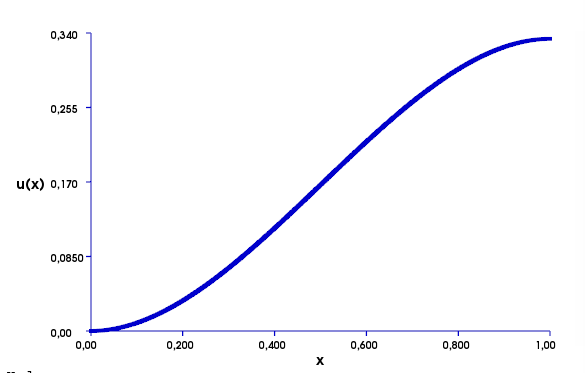
\includegraphics[width=0.5\textwidth]{fenics2.png}
\end{figure}

\begin{figure}[H]
  \caption{manufacture solution $t=2$}
  \centering
    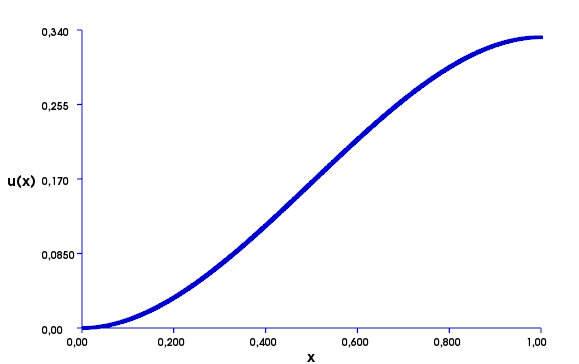
\includegraphics[width=0.5\textwidth]{an.png}
\end{figure}

\subsection{FENiCs Errors}



\subsection{Nonlinear verification}
The nonlinear FEniCs implementation is verified and the convergence rate of 1 is computed. See file name 
\textbf{nonLinearVerification.py}

\section{Simulation of the nonlinear Gaussian function}
The nonlinear Gaussian function 
\begin{equation}
I(x,y) = \exp\left(  -\frac{1}{2\sigma^{2}}(x^{2}+y^{2})  \right) \quad (x,y)\in [0,1]\times[0,1]
\end{equation}
simulation is given by the following figures

\begin{figure}[H]
  \caption{Nonlinear Gaussian function at $t=1$}
  \centering
    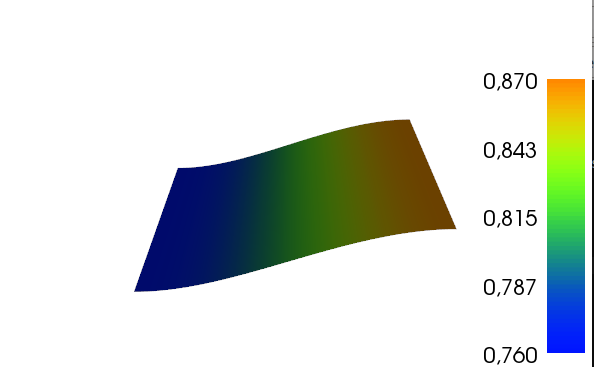
\includegraphics[width=0.5\textwidth]{g1.png}
\end{figure}

\begin{figure}[H]
  \caption{Nonlinear Gaussian function at $t=2$}
  \centering
    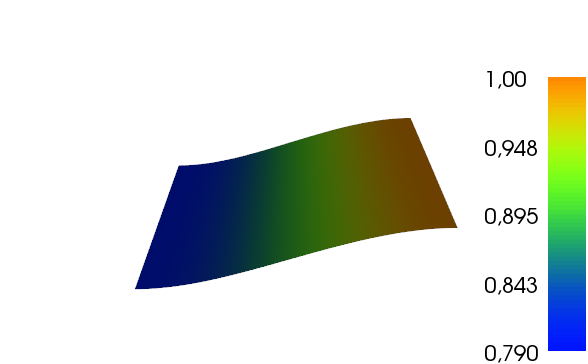
\includegraphics[width=0.5\textwidth]{g2.png}
\end{figure}

\begin{figure}[H]
  \caption{Nonlinear Gaussian function at $t=3$}
  \centering
    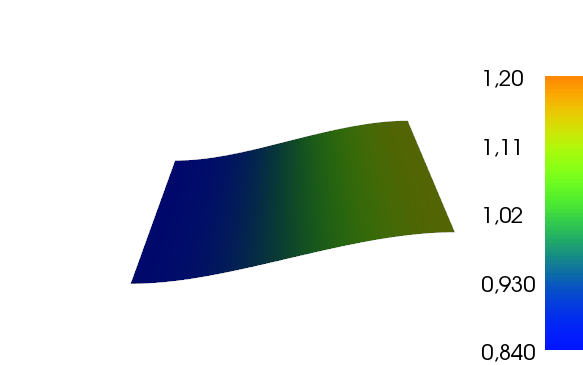
\includegraphics[width=0.5\textwidth]{g3.png}
\end{figure}

\end{document}